% This file was created by matlab2tikz.
%
%The latest updates can be retrieved from
%  http://www.mathworks.com/matlabcentral/fileexchange/22022-matlab2tikz-matlab2tikz
%where you can also make suggestions and rate matlab2tikz.
%
\definecolor{mycolor1}{rgb}{0.85000,0.95000,1.00000}%
\definecolor{mycolor2}{rgb}{0.95000,0.85000,0.85000}%
\definecolor{mycolor3}{rgb}{0.06600,0.44300,0.74500}%
\definecolor{mycolor4}{rgb}{0.12941,0.12941,0.12941}%
%
\begin{tikzpicture}

\begin{axis}[%
width=0.951\textwidth,
height=0.058\textheight,
at={(0\textwidth,0.162\textheight)},
scale only axis,
xmin=0,
xmax=159,
ymin=0,
ymax=394.8,
ylabel style={font=\color{mycolor4}},
ylabel={Packets/s},
axis background/.style={fill=white},
title style={font=\bfseries\color{mycolor4}},
title={toolbox-0 — sub-managed-1},
axis x line*=bottom,
axis y line*=left,
xmajorgrids,
ymajorgrids,
grid=both,
tick align=outside,
scaled y ticks=false
]

\addplot[area legend, draw=none, fill=mycolor1, fill opacity=0.35, forget plot]
table[row sep=crcr] {%
x	y\\
13	0\\
23	0\\
23	394.8\\
13	394.8\\
}--cycle;

\addplot[area legend, draw=none, fill=mycolor2, fill opacity=0.25, forget plot]
table[row sep=crcr] {%
x	y\\
38	0\\
43	0\\
43	394.8\\
38	394.8\\
}--cycle;
\addplot [color=mycolor3, forget plot]
  table[row sep=crcr]{%
0	0\\
22	0\\
23	6\\
24	10\\
32	10\\
33	4\\
34	0\\
137	0\\
139	40\\
141	40\\
142	376\\
143	2\\
144	0\\
145	0\\
146	2\\
148	2\\
149	0\\
150	2\\
151	0\\
152	2\\
153	0\\
155	0\\
156	4\\
157	0\\
159	0\\
};
\end{axis}

\begin{axis}[%
width=0.951\textwidth,
height=0.058\textheight,
at={(0\textwidth,0.081\textheight)},
scale only axis,
xmin=0,
xmax=159,
ymin=0,
ymax=12.6,
ylabel style={font=\color{mycolor4}},
ylabel={Packets/s},
axis background/.style={fill=white},
title style={font=\bfseries\color{mycolor4}},
title={toolbox-0 — sub-managed-2},
axis x line*=bottom,
axis y line*=left,
xmajorgrids,
ymajorgrids,
grid=both,
tick align=outside,
scaled y ticks=false
]

\addplot[area legend, draw=none, fill=mycolor1, fill opacity=0.35, forget plot]
table[row sep=crcr] {%
x	y\\
13	0\\
23	0\\
23	12.6\\
13	12.6\\
}--cycle;

\addplot[area legend, draw=none, fill=mycolor2, fill opacity=0.25, forget plot]
table[row sep=crcr] {%
x	y\\
38	0\\
43	0\\
43	12.6\\
38	12.6\\
}--cycle;
\addplot [color=mycolor3, forget plot]
  table[row sep=crcr]{%
0	0\\
22	0\\
23	7\\
24	10\\
25	10\\
26	11\\
27	10\\
28	10\\
29	12\\
30	12\\
31	10\\
32	12\\
33	4\\
34	0\\
141	0\\
142	2\\
143	0\\
146	0\\
147	4\\
148	0\\
159	0\\
};
\end{axis}

\begin{axis}[%
width=0.951\textwidth,
height=0.058\textheight,
at={(0\textwidth,0\textheight)},
scale only axis,
xmin=0,
xmax=159,
xlabel style={font=\color{mycolor4}},
xlabel={Time (s)},
ymin=0,
ymax=2.1,
ylabel style={font=\color{mycolor4}},
ylabel={Packets/s},
axis background/.style={fill=white},
title style={font=\bfseries\color{mycolor4}},
title={toolbox-1 — sub-managed-2},
axis x line*=bottom,
axis y line*=left,
xmajorgrids,
ymajorgrids,
grid=both,
tick align=outside,
scaled y ticks=false
]

\addplot[area legend, draw=none, fill=mycolor1, fill opacity=0.35, forget plot]
table[row sep=crcr] {%
x	y\\
13	0\\
23	0\\
23	2.1\\
13	2.1\\
}--cycle;

\addplot[area legend, draw=none, fill=mycolor2, fill opacity=0.25, forget plot]
table[row sep=crcr] {%
x	y\\
38	0\\
43	0\\
43	2.1\\
38	2.1\\
}--cycle;
\addplot [color=mycolor3, forget plot]
  table[row sep=crcr]{%
0	0\\
7	0\\
8	2\\
9	0\\
141	0\\
142	2\\
143	0\\
159	0\\
};
\end{axis}
\end{tikzpicture}%